\chapter{Requisiti Funzionali}
\label{ch:requisitiFunzionali}

Di seguito vengono riportati i requisiti funzionali (\texttt{RF}) del programma ``SatisTrento'' tramite \textit{Use Case Diagram} (\texttt{UCD}) progettati usando il linguaggio \texttt{UML}.

\section{\underline{Utente non loggato}}
    Di seguito i requisiti associati all'Utente non loggato:
    \begin{itemize}
        \item \textbf{RF1}: Visualizzare città
        \item \textbf{RF2}: Interagire con la mappa
        \item \textbf{RF3}: Visualizzare zona
        \item \textbf{RF4}: Visualizzare elenco strutture
        \item \textbf{RF5}: Multi lingua
        \item \textbf{RF6}: Login
    \end{itemize}
    \begin{figure}[H]
        \centering
        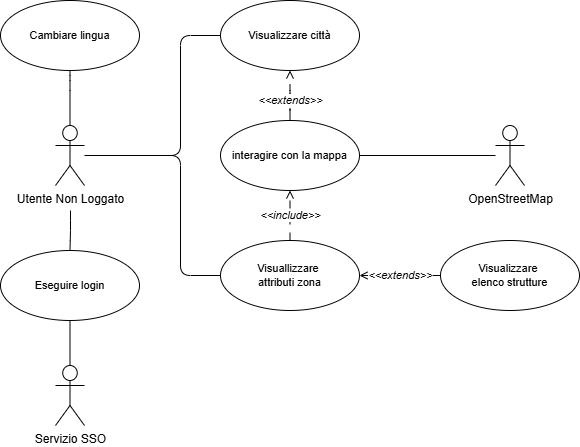
\includegraphics[width=0.8\textwidth]{UseCase_diagrams/NonLoggato.drawio.png}
        \caption{\textit{Use Case Diagram} dell'Utente non loggato}
    \end{figure}

    \subsection{\textit{Use Case} RF1: Visualizzare città}
        \subsubsection{Riassunto}
            Questo \textit{Use Case} descrive come l'utente può visualizzare gli attributi e la mappa della città
        \subsubsection{Descrizione}
            \begin{itemize}
                \item Il sistema mostra nella parte sinistra dello schermo gli attributi demografici e riguardanti la soddisfazione della città
                \item Il sistema mostra nella parte destra dello schermo la mappa della città suddivisa nella zona selezionata (Estensione 1)
            \end{itemize}
        \subsubsection{Estensioni}
            \begin{itemize}
                \item La tipologia di zona selezionata di default è quella dei quartieri
            \end{itemize}
    
    \subsection{\textit{Use Case} RF2: Interagire con la mappa}
        \subsubsection{Riassunto}
            Questo \textit{Use Case} descrive come l'utente può interagire con la mappa
        \subsubsection{Descrizione}
            \begin{itemize}
                \item L'utente non loggato posiziona il cursore all'interno dello spazio dedicato alla mappa
                \item Se l'utente utilizza la rotella del mouse oppure uno dei pulsanti presenti in uno degli angoli della mappa
                \item Attraverso le funzionalità fornite da \texttt{OpenStreetMap}\footnote{
                    \label{note:osm}
                    $ \text{\texttt{OpenStreetMap}}^{\text{\textregistered}} $ è basato su \textit{dati aperti}, rilasciato con licenza \href{https://opendatacommons.org/licenses/odbl/}{\textit{Open Data Commons Open Database License} (\texttt{ODbL})} da \href{https://osmfoundation.org/}{\textit{\texttt{OpenStreetMap} Foundation} (\texttt{OSMF})}. Per ulteriori informazioni si rimanda al sito ufficiale: \url{https://www.openstreetmap.org/}
                } la mappa ingrandisce o diminuisce la dimensione dello zoom (Eccezione 1)
                \item Se l'utente preme e trascina il cursore
                \item Attraverso le funzionalità fornite da \texttt{OpenStreetMap}\footref{note:osm} la mappa sposta il focus centrale in funzione del cursore (Eccezione 2)
                \item Se l'utente non loggato seleziona una delle zone all'interno della visuale della mappa (Estensione 1)
                \item Il sistema posiziona il focus centrale della mappa al centro della zona selezionata e ne modifica successivamente lo zoom, il colore e lo spessore dei bordi
                \item Il sistema passa successivamente allo \textit{Use Case} ``Visualizzare zona'' della sezione scelta(Eccezione 3)
            \end{itemize}
        \subsubsection{Eccezioni}
            \begin{enumerate}
                \item Nel caso in cui l'utente non loggato cercasse di aumentare o diminuire lo zoom oltre ai limiti imposti, il sistema deve bloccare la nuova modifica allo zoom
                \item Nel caso in cui l'utente non loggato cercasse di spostare il focus centrale oltre ai limiti della città, il sistema deve bloccare la nuova modifica allo spostamento del focus centrale
                \item Nel caso in cui l'utente avesse i permessi necessari, il sistema passerà allo \textit{Use Case} ``Visualizzare attributi completi'' della sezione scelta invece che allo allo \textit{Use Case} ``Visualizzare zona'' della sezione scelta
            \end{enumerate}
        \subsubsection{Estensioni}
            \begin{enumerate}
                \item Nel caso in cui l'utente cliccasse su di una zona già selezionata questa riporterebbe allo \textit{Use Case} ``Visualizzare città''
                \item L'utente, selezionando il pulsante presente nell'angolo della mappa, potrà visualizzare un menù pop-up e successivamente modificare la tipologia di zona visualizzabile all'interno della mappa.
                Nel caso in cui l'utente avesse i permessi necessari, sarà inoltre possibile cambiare la tipologia di visualizzazione da mappa a tabella.
            \end{enumerate}
    
    \subsection{\textit{Use Case} RF3: Visualizzare zona}
        \subsubsection{Riassunto}
            Questo \textit{Use Case} descrive come l'utente può visualizzare la zona selezionata della città
        \subsubsection{Descrizione}
            \begin{enumerate}
                \item L'utente seleziona una zona geografica per la quale ricevere maggiori informazioni
                \item Il sistema mostra nella parte sinistra dello schermo la mappa centrata sul centro della zona selezionata
                \item Il sistema mostra nella parte destra dello schermo gli attributi demografici e riguardanti la soddisfazione della zona della città selezionata
            \end{enumerate}

    \subsection{\textit{Use Case} RF4: Visualizzare elenco strutture}
        \subsubsection{Riassunto}
            Questo \textit{Use Case} descrive come l'utente può accedere e visualizzare l'elenco delle strutture che forniscono un servizio al cittadino
        \subsubsection{Descrizione}
            \begin{enumerate}
                \item Se l'utente seleziona uno degli attributi presenti a schermo (Eccezione 1)
                \item Il sistema presenta a schermo, ove prima erano presenti gli attributi riguardanti la zona selezionata, una tabella contenente una lista numerata di strutture che offrono il servizio selezionato in precedenza
                \item Il sistema deve successivamente segnalare sulla mappa la posizione delle varie strutture, attraverso un segnalino contenente il numero identificativo presente in tabella della struttura
            \end{enumerate}
        \subsubsection{Eccezioni}
            \begin{enumerate}
                \item Nel caso in cui per una tipologia di dato non fossero presenti strutture il sistema non deve fare nulla
            \end{enumerate}
        \subsubsection{Estensioni}
            \begin{enumerate}
                \item Nel caso in cui l'utente cliccasse il pulsante per chiudere la tabella il sistema tornerà alla visualizzazione della zona selezionata in precedenza
            \end{enumerate}

    \subsection{\textit{Use Case} RF5: Cambiare lingua}
        \subsubsection{Riassunto}
            Questo \textit{Use Case} descrive come l'utente può cambiare la lingua dei vari testi presenti nel programma
        \subsubsection{Descrizione}
            \begin{enumerate}
                \item L'utente preme sul menù a tendina presente nella header e seleziona la sezione riguardante la modifica della lingua
                \item Il sistema presenterà a schermo un menù pop-up contenente la lista di lingue per le quali è disponibile la traduzione
                \item Se l'utente seleziona la lingua e clicca il pulsante di conferma (Eccezione 1 e 2)
                \item Il sistema ricarica la pagina selezionata con i testi nella lingua selezionata
            \end{enumerate}
        \subsubsection{Eccezioni}
            \begin{enumerate}
                \item Nel caso in cui l'utente non loggato selezionasse e confermasse la lingua già selezionata, il sistema deve chiudere il pop-up senza apportare alcuna modifica
            \end{enumerate}

    \subsection{\textit{Use Case} RF6: Eseguire login}
        \subsubsection{Riassunto}
            Questo \textit{Use Case} descrive come l'utente non loggato può eseguire il login
        \subsubsection{Descrizione}
            \begin{enumerate}
                \item L'utente preme sul menù a tendina presente all'interno della header e seleziona la sezione riguardante il login
                \item Il sistema reindirizza l'utente alla pagina del service provider della provincia di Trento dal quale potrà accedere al login tramite sistema \texttt{SSO}
                \item Il sistema \texttt{SSO} verifica l'identità dell'utente in questione e la ritorna al sistema (Eccezione 1)
                \item Il sistema controlla che per l'identità certificata dal sistema \texttt{SSO} esista un'account collegato (Eccezione 1)
                \item Il sistema assegna dunque un'identità all'utente assegnandogli il ruolo di proprietà
                \item Il sistema successivamente al login sostituisce l'icona del login con l'immagine profilo dell'account al quale si ha fatto l'accesso e reindirizza l'utente allo \textit{Use Case} ``visualizzare città''
            \end{enumerate}
        \subsubsection{Eccezioni}
            \begin{enumerate}
                \item Nel caso in cui l'autenticazione fallisse o non vi fossero account collegati il sistema ritorna alla pagina del login segnalando l'errore
            \end{enumerate}


\section{\underline{Utente sondaggista}}
    Di seguito i requisiti associati all'Utente sondaggista:
    \begin{itemize}
        \item \textbf{RF7}: Eseguire logout
        \item \textbf{RF8}: Visualizzare i sondaggi
        \item \textbf{RF9}: Gestire i sondaggi
        \item \textbf{RF10}: Visualizzare i voti
        \item \textbf{RF11}: Gestire i voti
    \end{itemize}
    \begin{figure}[H]
        \centering
        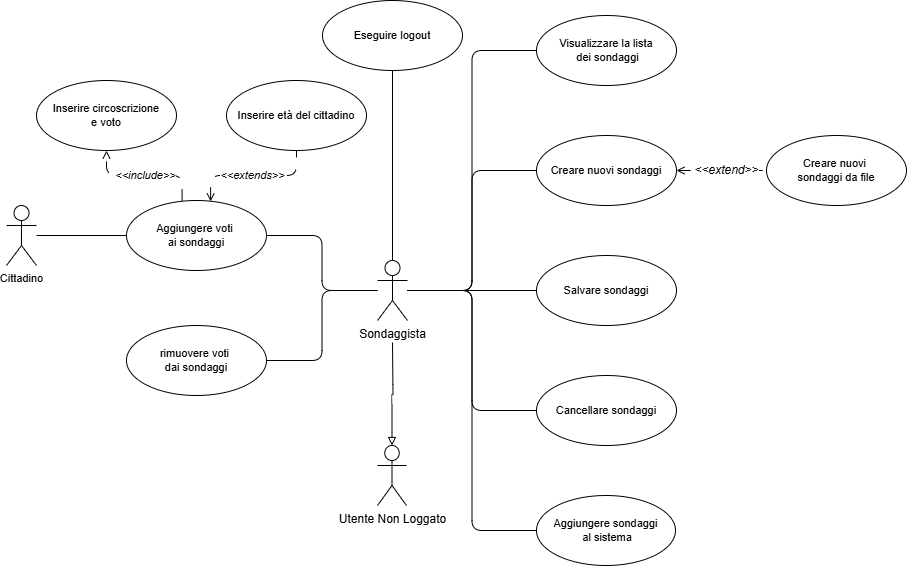
\includegraphics[width=1\textwidth]{UseCase_diagrams/Sondaggista.drawio.png}
        \caption{\textit{Use Case Diagram} dell'Utente sondaggista}
    \end{figure}

    \subsection{\textit{Use Case} RF7: Eseguire logout}
        \subsubsection{Riassunto}
            Questo \textit{Use Case} descrive come l'utente può fare logout
        \subsubsection{Descrizione}
            \begin{enumerate}
                \item L'utente sondaggista preme sul menù a tendina presente all'interno della header e seleziona la sezione riguardante il logout
                \item Il sistema scollega lo user dall'account al quale era collegato riportandolo allo stato di utente non loggato, infine 
                ricarica la pagina riportando l'utente allo \textit{Use Case} ``visualizzare città''
            \end{enumerate}

    \subsection{\textit{Use Case} RF8: Visualizzare i sondaggi}
        \subsubsection{Riassunto}
            Questo \textit{Use Case} descrive come l'utente sondaggista può visualizzare i sondaggi e le interfacce per gestirli
        \subsubsection{Descrizione}
            \begin{enumerate}
                \item Il sistema mostra nel riquadro in alto a sinistra dello schermo l'interfaccia per la creazione di nuovi sondaggi con relative caselle di testo e pulsante per la creazione
                \item Il sistema mostra nel riquadro in basso a sinistra dello schermo l'interfaccia per il caricamento dei sondaggi attraverso pulsante o ``\textit{drag and drop}''
                \item Il sistema mostra nel riquadro in alto a destra dello schermo l'elenco dei sondaggi non ancora caricati, o in fase di caricamento, a sistema con relativo stato della sessione (Eccezione 1)
                \item Il sistema mostra nel riquadro in basso a destra dello schermo l'elenco dei sondaggi già caricati a sistema con relativo stato di caricamento e stato di verifica dei dati inseriti (Eccezione 1)
            \end{enumerate}
        \subsubsection{Eccezioni}
            \begin{enumerate}
                \item Nel caso in cui non fossero presenti sondaggi all'interno di uno degli elenchi il sistema mostrerà a schermo un messaggio per avvisare che tale sezione risulta vuota
            \end{enumerate}

    \subsection{\textit{Use Case} RF9: Gestire i sondaggi}
        \subsubsection{Riassunto}
            Questo \textit{Use Case} descrive come l'utente può gestire i sondaggi
             \begin{figure}[H]
                 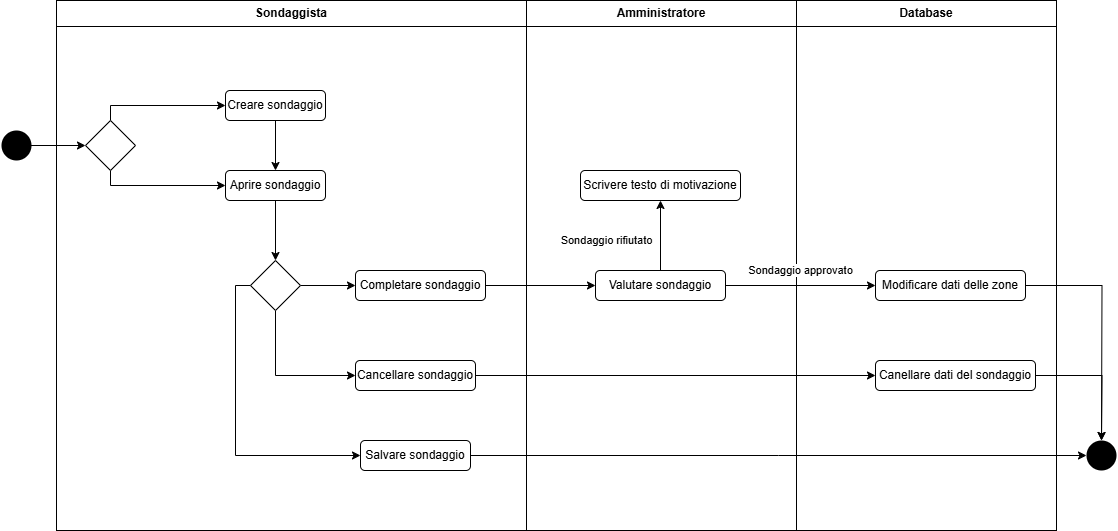
\includegraphics[width=0.9\textwidth]{ActivityDiagrams/ActivityDiagram_RF9.drawio.png}
             \end{figure}

    \subsection{\textit{Use Case} RF10: Visualizzare i voti}
        \subsubsection{Riassunto}
            Questo \textit{Use Case} descrive come l'utente sondaggista può visualizzare i voti e le interfacce per gestirli
        \subsubsection{Descrizione}
            \begin{enumerate}
                \item Il sistema mostra nella parte sinistra dello schermo un riassunto del numero di voti presenti all'interno del sondaggio e in basso una tabella riassuntiva riguardante il numero di voti ricevuti per quartiere
                \item Il sistema mostra nel riquadro in alto a destra dello schermo l'interfaccia per il caricamento dei voti con le corrispettive caselle di testo
                \item Il sistema mostra nel riquadro in basso a destra dello schermo l'interfaccia per la gestione dei sondaggi
                \item Il sistema mostra nel riquadro in basso al centro dello schermo l'elenco dei voti caricati in precedenza, su ogni voto è inoltre presente l'id, l'ora al quale è stato caricato il voto e infine il pulsante per eliminarlo (Eccezione 1)
            \end{enumerate}
        \subsubsection{Eccezioni}
            \begin{enumerate}
                \item Nel caso in cui non fossero presenti voti all'interno della lista il sistema mostrerà a schermo un messaggio per avvisare che tale sezione risulta vuota
            \end{enumerate}

    \subsection{\textit{Use Case} RF11: Gestire i voti}
        \subsubsection{Riassunto}
            Questo \textit{Use Case} descrive come l'utente può gestire i voti
             \begin{figure}[H]
                 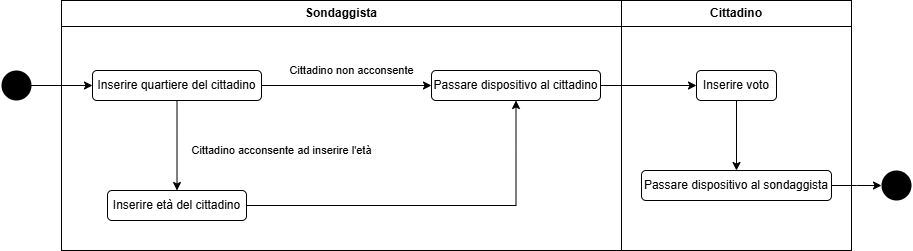
\includegraphics[width=0.9\textwidth]{ActivityDiagrams/ActivityDiagram_RF11.drawio.png}
             \end{figure}


\section{\underline{Utente analista}}
    Di seguito i requisiti associati all'Utente analista:
    \begin{itemize}
        \item \textbf{RF7}: Eseguire logout
        \item \textbf{RF12}: Interagire con la tabella
        \item \textbf{RF13}: Visualizzare attributi completi
        \item \textbf{RF14}: Analizzare storico dei dati
    \end{itemize}
    \begin{figure}[H]
        \centering
        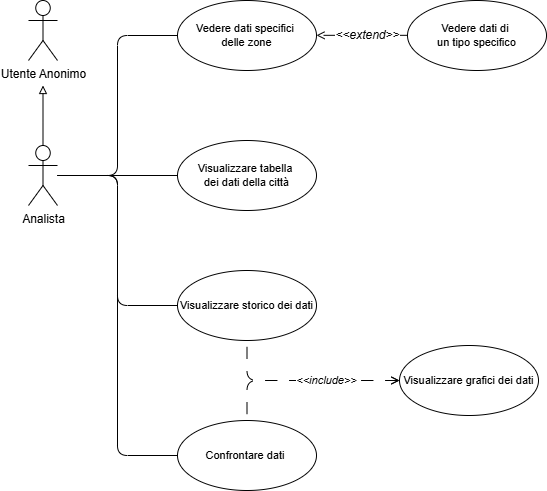
\includegraphics[width=0.7\textwidth]{UseCase_diagrams/Analista.drawio.png}
        \caption{\textit{Use Case} Diagram dell'Utente analista}
    \end{figure}

    \subsection{\textit{Use Case} RF7: Eseguire logout}
        \subsubsection{Riassunto}
            Questo \textit{Use Case} descrive come l'utente può fare logout
        \subsubsection{Descrizione}
            \begin{enumerate}
                \item L'utente analista preme sul menù a tendina presente all'interno della header e seleziona la sezione riguardante il logout
                \item Il sistema scollega lo user dall'account al quale era collegato riportandolo allo stato di utente non loggato, infine 
                ricarica la pagina riportando l'utente allo \textit{Use Case} ``visualizzare città''
            \end{enumerate}

    \subsection{\textit{Use Case} RF12: Interagire con la tabella}
        \subsubsection{Riassunto}
            Questo \textit{Use Case} descrive come l'utente analista visualizzerà e potrà interagire con la tabella
        \subsubsection{Descrizione}
            \begin{enumerate}
                \item L'utente analista posiziona il cursore all'interno dello spazio dedicato alla tabella
                \item Se l'utente utilizza la rotella del mouse
                \item La tabella scorre gli elementi presenti all'interno della tabella (Eccezione 1)
                \item Se l'utente seleziona uno degli attibuti all'interno della riga di intestazione della tabella
                \item Il sistema ordina le tuple presenti all'interno della tabella in base al dominio dell'attributo
                \item Se l'utente seleziona l'attributo contenente il nome di una delle zone presenti all'interno del comune
                \item Il sistema passa dalla visualizzazione tramite tabella a quella tramite mappa
                \item il sistema sposta il focus centrale della mappa al centro della zona selezionata e ne modifica successivamente lo zoom, il colore e lo spessore dei bordi
                \item Il sistema passa successivamente allo \textit{Use Case} ``visualizzare attributi completi'' della sezione scelta
            \end{enumerate}
        \subsubsection{Eccezioni}
            \begin{enumerate}
                \item Nel caso in cui l'utente analista cercasse di scorrere gli elementi della lista oltre ai limiti imposti, il sistema deve bloccare il nuovo tentativo di scorrimento
            \end{enumerate}
        \subsubsection{Estensioni}
            \begin{enumerate}
                \item L'utente, selezionando il pulsante presente nell'angolo della tabella, potrà visualizzare un menù pop-up.Successivamente potrà modificare la tipologia di zona presente all'interno della tabella oppure cambiare la tipologia di visualizzazione da tabella a mappa
            \end{enumerate}

    \subsection{\textit{Use Case} RF13: Visualizzare attributi completi}
        \subsubsection{Riassunto}
            Questo \textit{Use Case} descrive come l'utente analista può visualizzare, accedere e navigare agli attributi completi riguardanti ogni zona
        \subsubsection{Descrizione}
            \begin{enumerate}
                \item L'utente seleziona una zona geografica per la quale ricevere maggiori informazioni
                \item Il sistema mostra nella parte sinistra dello schermo la mappa centrata sul centro della zona selezionata
                \item Il sistema mostra nella parte destra dello schermo la categoria di attributi riguardanti la zona selezionata con al di sopra le icone ed il titolo delle varie categorie di attributi selezionabili (Estensione 2)
                \item L'utente seleziona la categoria di attributi che vuole visualizzare (Eccezione 1)
                \item Il sistema mostra, ove prima erano presenti gli attributi della precedente categoria, gli attributi appartenenti alla nuova categoria selezionata
            \end{enumerate}
        \subsubsection{Eccezioni}
            \begin{enumerate}
                \item Se si seleziona la categoria di attributi già selezionata il sistema non deve fare nulla
            \end{enumerate}
        \subsubsection{Estensioni}
            \begin{enumerate}
                \item Questo \textit{Use Case} estende lo \textit{Use Case} ``Visualizzare Zona'' dell'utente non loggato
                \item La categoria di attributi selezionata di default è quella degli attributi generali
            \end{enumerate}

    \subsection{\textit{Use Case} RF14: Analizzare storico dei dati}
        \subsubsection{Riassunto}
            Questo \textit{Use Case} descrive come l'utente analista può visualizzare e interagire con gli storici
        \subsubsection{Descrizione}
            \begin{enumerate}
                \item Il sistema mostra a fianco degli attributi presenti all'interno dello \textit{Use Case} ``Visualizzare attributi completi'' il grafico rappresentante l'andamento nel tempo di tale attributo
                \item L'utente seleziona il grafico
                \item Il sistema sposta l'attributo selezionato e successivamente posiziona al centro il grafico modificandone le dimensioni (Eccezione 1)
                \item Se l'utente posiziona il cursore all'interno del grafico
                \item Il sistema mostrerà tramite messaggio a comparsa lo stato dell'attributo nell'istante di tempo selezionato
            \end{enumerate}
        \subsubsection{Eccezioni}
            \begin{enumerate}
                \item Nel caso in cui per un'attributo non fossero reperibili sufficienti dati non sarà presente la propria rappresentazione tramite grafico
            \end{enumerate}


\section{\underline{Utente circoscrizione}}
    Di seguito i requisiti associati all'Utente circoscrizione:
    \begin{itemize}
        \item \textbf{RF7}: Eseguire logout
        \item \textbf{RF15}: Visualizzare richieste
        \item \textbf{RF16}: Gestire richieste
        \item \textbf{RF17}: Gestire ruoli Circoscrizione
        \item \textbf{RF18}: Modificare informazioni servizi Circoscrizione
    \end{itemize}
    \begin{figure}[H]
        \centering
        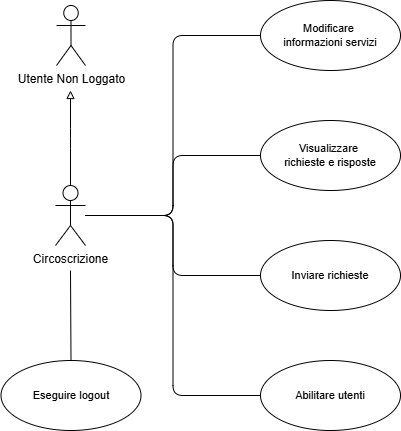
\includegraphics[width=1\textwidth]{UseCase_diagrams/Circoscrizione.drawio.png}
        \caption{\textit{Use Case} Diagram dell'Utente circoscrizione}
    \end{figure}

    \subsection{\textit{Use Case} RF7: Eseguire logout}
        \subsubsection{Riassunto}
            Questo \textit{Use Case} descrive come l'utente può fare logout
        \subsubsection{Descrizione}
            \begin{enumerate}
                \item L'utente circoscrizione preme sul menù a tendina presente all'interno della header e seleziona la sezione riguardante il logout
                \item Il sistema scollega lo user dall'account al quale era collegato riportandolo allo stato di utente non loggato, infine 
                ricarica la pagina riportando l'utente allo \textit{Use Case} ``visualizzare città''
            \end{enumerate}

    \subsection{\textit{Use Case} RF15: Visualizzare richieste}
        \subsubsection{Riassunto}
            Questo \textit{Use Case} descrive come l'utente circoscrizione può visualizzare le richieste e le interfacce per gestirle
        \subsubsection{Descrizione}
            \begin{enumerate}
                \item L'utente preme sul menù a tendina presente nella header e seleziona il campo riguardante le richieste agli amministratori
                \item Il sistema mostra nella parte sinistra dello schermo l'interfaccia per l'aggiunta di una nuova richiesta
                \item Il sistema mostra nel riquadro in alto a destra dello schermo l'elenco delle richieste inviate agli Utenti amministratore per le quali non è ancora stata ricevuta una risposta (Eccezione 1)
                \item Il sistema mostra nel riquadro in basso a destra dello schermo l'elenco delle richieste per le quali è già stata ricevuta una risposta (Eccezione 1)
            \end{enumerate}
        \subsubsection{Eccezioni}
            \begin{enumerate}
                \item Nel caso in cui non fossero presenti richieste all'interno di uno degli elenchi il sistema mostrerà a schermo un messaggio per avvisare che tale sezione risulta vuota
            \end{enumerate}

    \subsection{\textit{Use Case} RF16: Gestire richieste}
        \subsubsection{Riassunto}
            Questo \textit{Use Case} descrive come l'utente può gestire le richieste per gli Utenti ammisistratore
        \subsubsection{Descrizione}
            \begin{enumerate}
                \item Se l'utente circoscrizione completa gli appositi campi di testo e conferma attraverso il pulsante apposito (Eccezione 1)
                \item Il sistema invia il messaggio agli utenti amministratore tenendo traccia della circoscrizione di provenienza, del titolo e del corpo del messaggio
                \item Il sistema aggiunge la nuova richiesta alla lista delle richieste per le quali non è ancora stata ricevuta una risposta
                \item Se l'utente seleziona una delle richieste all'interno di uno degli elenchi
                \item Il sistema presenta al centro dello schermo tramite pop up il titolo ed il corpo della richiesta (Estensione 1)
                \item Se l'utente seleziona una delle richieste e seleziona il pulsante per eliminare la richiesta (Eccezione 2)
                \item Il sistema mostra a schemo un pop up per confermare tale azione
                \item Se l'utente conferma la decisione (Eccezione 3)
                \item Il sistema elimina la richiesta e riporta l'utente allo \textit{Use Case} ``Visualizzare richieste''
            \end{enumerate}
        \subsubsection{Eccezioni}
            \begin{enumerate}
                \item Nel caso in cui l'utente selezionasse il pulsante di conferma prima di aver riempito i campi necessari, comparirà a schermo un messaggio di errore e l'azione di invio della richiesta verrà bloccata
                \item Nel caso in cui la richiesta avesse già ricevuto una risposta non sarà più presente a schermo il pulsante per eliminare supposta richiesta
                \item Nel caso in cui l'utente non confermasse la decisione di eliminare la richiesta verrebbe reindirizzato alla visualizzazione della richiesta selezionata in precedenza e il processo di eliminazione verrebbe bloccato
            \end{enumerate}
        \subsubsection{Estensioni}
            \begin{enumerate}
                \item Nel caso in cui per la richiesta selezionata fosse disponibile la risposta da parte di un utente amministratore tale messaggio verrebbe presentato al seguito del messaggio di richiesta 
            \end{enumerate}

    \subsection{\textit{Use Case} RF17: Gestire ruoli Circoscrizione}
        \subsubsection{Riassunto}
            Questo \textit{Use Case} descrive come l'utente circoscrizione può gestire i ruoli all'interno della propria circoscrizione
        \subsubsection{Descrizione}
            \begin{enumerate}
                \item L'utente preme sul menù a tendina presente nella header e seleziona il campo riguardante la gestione dei ruoli
                \item L'utente circoscrizione inserisce all'interno dell'apposito spazio di testo il codice fiscale dell'utente interessato
                \item Il sistema presenta a schermo le informazioni dell'utente selezionato (Eccezione 1)
                \item Se l'utente seleziona la tipologia di ruolo che si vuole assegnare e seleziona il pulsante di conferma (Eccezione 2)
                \item Il sistema fornisce all'utente il ruolo selezionato in precedenza con validità limitata alla circoscrizione di appartenenza (Eccezione 3)
                \item Se l'utente seleziona il pulsante di rimozione ruolo a fianco del ruolo desiderato e seleziona il pulsante di conferma
                \item Il sistema rimuove all'utente selezionato il ruolo scelto (Eccezione 4)
            \end{enumerate}
        \subsubsection{Eccezioni}
            \begin{enumerate}
                \item Nel caso in cui il Codice Fiscale cercato non fosse collegato ad alcun account il sistema deve presentare un messaggio di errore
                \item Nel caso in cui non venisse selezionato alcun ruolo e venisse selezionato il pulsante di conferma il sistema non deve fare nulla
                \item Nel caso in cui l'utente fosse già in possesso del ruolo selezionato il sistema non deve fare nulla
                \item Nel caso in cui l'utente provasse a rimuovere un ruolo sul quale non ha possibilità di modifica il tentativo di modifica viene bloccato
            \end{enumerate}

    \subsection{\textit{Use Case} RF18: Modificare informazioni servizi Circoscrizione}
        \subsubsection{Riassunto}
        Questo \textit{Use Case} descrive come l'utente può modificare le informazioni riguardanti i servizi presenti all'interno della circoscrizione
        \subsubsection{Descrizione}
            \begin{enumerate}
                \item L'utente preme sul menù a tendina presente nella header e seleziona il campo riguardante la modifica delle informazioni
                \item Se l'utente circoscrizione completa gli appositi campi di testo obbligatori e conferma attraverso il pulsante apposito (Eccezione 1)
                \item Il sistema propaga l'aggiunta del servizio all'interno dell'elenco dei servizi dell'apposita circoscrizione
                \item Se l'utente seleziona uno dei servizi all'interno dell'elenco dei servizi della circoscrizione
                \item Il sistema presenta al centro dello schermo i dati forniti al momento della registrazione del servizio
                \item Se l'utente modifica uno dei dati riguardanti il servizio
                \item Il sistema propaga la modifica all'interno dell'elenco dei servizi (Eccezione 2)
                \item Se l'utente seleziona il pulsante per eliminare il servizio
                \item Il sistema mostra a schemo un pop up per confermare tale azione
                \item Se l'utente conferma la decisione (Eccezione 3)
                \item Il sistema propaga l'eliminazione all'interno dell'elenco dei servizi
            \end{enumerate}
        \subsubsection{Eccezioni}
            \begin{enumerate}
                \item Nel caso in cui l'utente selezionasse il pulsante di conferma prima di aver riempito i campi obbligatori, comparirà a schermo un messaggio di errore e l'azione di aggiunta del servizio verrà bloccata
                \item Nel caso in cui la modifica rompesse qualche vincolo di dominio dei campi la modifica verrebbe annullata
                \item Nel caso in cui l'utente non confermasse la decisione di eliminare il servizio verrebbe reindirizzato alla visualizzazione del servizio selezionato in precedenza e il processo di eliminazione verrebbe bloccato
            \end{enumerate}


\section{\underline{Utente amministratore}}
    Di seguito i requisiti associati all'Utente amministratore:
    \begin{itemize}
        \item \textbf{RF7}: Eseguire logout
        \item \textbf{RF19}: Valutare sondaggi
        \item \textbf{RF20}: Gestire richieste dalle circoscrizioni
        \item \textbf{RF21}: Gestire ruoli
        \item \textbf{RF22}: Modificare informazioni servizi
    \end{itemize}
    \begin{figure}[H]
        \centering
        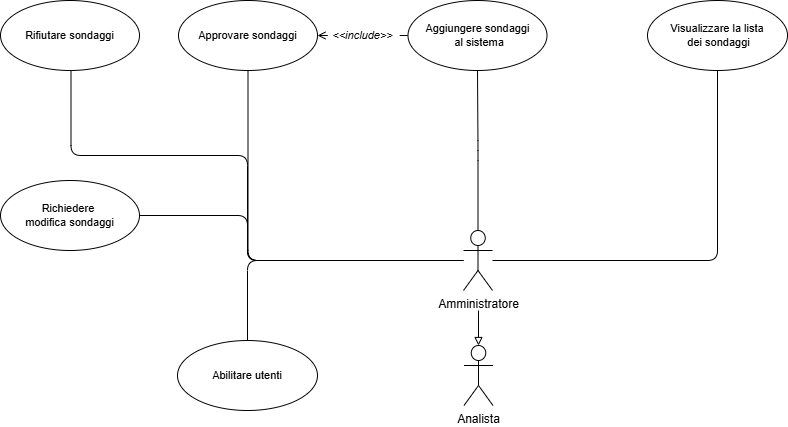
\includegraphics[width=0.9\textwidth]{UseCase_diagrams/Amministratore.drawio.png}
        \caption{\textit{Use Case} Diagram dell'Utente amministratore}
    \end{figure}

    \subsection{\textit{Use Case} RF7: Eseguireogout}
        \subsubsection{Riassunto}
            Questo \textit{Use Case} descrive come l'utente può fare logout
        \subsubsection{Descrizione}
            \begin{enumerate}
                \item L'utente amministratore preme sul menù a tendina presente all'interno della header e seleziona la sezione riguardante il logout
                \item Il sistema scollega lo user dall'account al quale era collegato riportandolo allo stato di utente non loggato, infine 
                ricarica la pagina riportando l'utente allo \textit{Use Case} ``visualizzare città''
            \end{enumerate}

    \subsection{\textit{Use Case} RF19: Valutare sondaggi}
        \subsubsection{Riassunto}
            Questo \textit{Use Case} descrive come l'utente amministratore può valutare i sondaggi 
        \subsubsection{Descrizione}
            \begin{enumerate}
                \item L'utente preme sul menù a tendina presente nella header e seleziona il campo riguardante la valutazione dei sondaggi
                \item Il sistema mostra l'elenco dei sondaggi in attesa (Eccezione 1)
                \item Se l'utente seleziona un sondaggio
                \item Il sistema mostra a schermo i dati completi riguardanti il sondaggio selezionato e una lista contenente lo stato dei sondaggi precedentemente caricati dal sondaggista (Eccezione 1)
                \item Il sistema mostra a schermo i pulsanti di apporvazione o disapprovazione del sondaggio
                \item Se l'utente approva il sondaggio
                \item Il sistema aggiunge i voti presenti nel sondaggio a sistema e rimuove il sondaggio dall'elenco dei sondaggi in attesa
                \item Se l'utente compila i campi appositi e rifiuta il sondaggio (Eccezione 2)
                \item Il sistema non aggiungei voti presenti nel sondaggio a sistema e restituisce la motivazione al sondaggista di riferimento
            \end{enumerate}
        \subsubsection{Eccezioni}
            \begin{enumerate}
                \item Nel caso in cui non fossero presenti sondaggi all'interno di uno degli elenchi il sistema mostrerà a schermo un messaggio per avvisare che tale sezione risulta vuota
                \item Nel caso in cui l'utente amministratore non compilasse il campo ``motivazione'' il sistema bloccherà il rifiuto del sondaggio e comparirà un messaggio di errore a schermo
            \end{enumerate}

    \subsection{\textit{Use Case} RF20: Gestire richieste dalle circoscrizioni}
        \subsubsection{Riassunto}
            Questo \textit{Use Case} descrive come l'utente amministratore può gestire le richieste da parte degli Utenti circoscrizione
        \subsubsection{Descrizione}
            \begin{enumerate}
                \item L'utente preme sul menù a tendina presente nella header e seleziona il campo riguardante la gestione delle richieste
                \item Il sistema mostra l'elenco delle richieste che non hanno ancora ricevuto una risposta (Eccezione 1)
                \item Se l'utente seleziona una richiesta
                \item Il sistema mostra a schermo il titolo e il corpo della richiesta, le informazioni riguardanti la circoscrizione dalla quale è stata inviata la richiesta e l'interfaccia di risposta
                \item Se l'utente compila i campi appositi e conferma l'invio della risposta (Eccezione 2)
                \item Il sistema invia la risposta agli utenti circoscrizione appositi e rimuove la richiesta dall'elenco delle richieste che non hanno ancora ricevuto una risposta
            \end{enumerate}
        \subsubsection{Eccezioni}
            \begin{enumerate}
                \item Nel caso in cui non fossero presenti richieste all'interno di uno degli elenchi il sistema mostrerà a schermo un messaggio per avvisare che tale sezione risulta vuota
                \item Nel caso in cui l'utente selezionasse il pulsante di invio prima di aver riempito i campi necessari, comparirà a schermo un messaggio di errore e l'azione di invio verrà bloccata
            \end{enumerate}

    \subsection{\textit{Use Case} RF21: Gestire ruoli}
        \subsubsection{Riassunto}
            Questo \textit{Use Case} descrive come l'utente amministratore può gestire i ruoli
        \subsubsection{Descrizione}
            \begin{enumerate}
                \item L'utente preme sul menù a tendina presente nella header e seleziona il campo riguardante la gestione dei ruoli
                \item L'utente amministratore inserisce all'interno dell'apposito spazio di testo il codice fiscale dell'utente interessato
                \item Il sistema presenta a schermo le informazioni dell'utente selezionato (Eccezione 1)
                \item Se l'utente seleziona la tipologia di ruolo che si vuole assegnare e seleziona il pulsante di conferma (Eccezione 2)
                \item Il sistema fornisce all'utente il ruolo selezionato in precedenza (Eccezione 3)
                \item Se l'utente seleziona il pulsante di rimozione ruolo a fianco del ruolo desiderato e seleziona il pulsante di conferma
                \item Il sistema rimuove all'utente selezionato il ruolo scelto (Estensione 1)
            \end{enumerate}
        \subsubsection{Eccezioni}
            \begin{enumerate}
                \item Nel caso in cui il Codice Fiscale cercato non fosse collegato ad alcun account il sistema deve presentare un messaggio di errore
                \item Nel caso in cui non venisse selezionato alcun ruolo e venisse selezionato il pulsante di conferma il sistema non deve fare nulla
                \item Nel caso in cui l'utente fosse già in possesso del ruolo selezionato il sistema non deve fare nulla
            \end{enumerate}
        \subsubsection{Estensioni}
            \begin{enumerate}
                \item La rimozione del ruolo da parte di un utente amministratore ha successo anche nel caso in cui il ruolo fosse stato assegnato da parte di una circoscrizione o da parte di un'altro account amministratore
                \item Questo \textit{Use Case} estende lo \textit{Use Case} ``Gestire ruoli Circoscrizione'' dell'utente circoscrizione
            \end{enumerate}

    \subsection{\textit{Use Case} RF22: Modificare informazioni servizi}
        \subsubsection{Riassunto}
        Questo \textit{Use Case} descrive come l'utente può modificare le informazioni riguardanti i servizi
        \subsubsection{Descrizione}
            \begin{enumerate}
                \item L'utente preme sul menù a tendina presente nella header e seleziona il campo riguardante la modifica delle informazioni
                \item Se l'utente amministratore completa gli appositi campi di testo obbligatori e conferma attraverso il pulsante apposito (Eccezione 1)
                \item Il sistema propaga l'aggiunta del servizio all'interno dell'elenco dei servizi della circoscrizione selezionata precedentemente
                \item Se l'utente seleziona uno dei servizi all'interno dell'elenco dei servizi
                \item Il sistema presenta al centro dello schermo i dati forniti al momento della registrazione del servizio
                \item Se l'utente modifica uno dei dati riguardanti il servizio
                \item Il sistema propaga la modifica all'interno dell'elenco dei servizi (Eccezione 2)
                \item Se l'utente seleziona il pulsante per eliminare il servizio
                \item Il sistema mostra a schemo un pop up per confermare tale azione
                \item Se l'utente conferma la decisione (Eccezione 3)
                \item Il sistema propaga l'eliminazione all'interno dell'elenco dei servizi
            \end{enumerate}
        \subsubsection{Eccezioni}
            \begin{enumerate}
                \item Nel caso in cui l'utente selezionasse il pulsante di conferma prima di aver riempito i campi obbligatori, comparirà a schermo un messaggio di errore e l'azione di aggiunta del servizio verrà bloccata
                \item Nel caso in cui la modifica rompesse qualche vincolo di dominio dei campi la modifica verrebbe annullata
                \item Nel caso in cui l'utente non confermasse la decisione di eliminare il servizio verrebbe reindirizzato alla visualizzazione del servizio selezionato in precedenza e il processo di eliminazione verrebbe bloccato
            \end{enumerate}
        \subsubsection{Estensioni}
            \begin{enumerate}
                \item Questo \textit{Use Case} estende lo \textit{Use Case} ``Modificare informazioni servizi Circoscrizione'' dell'utente circoscrizione
            \end{enumerate}
